While analyzing RNA-Seq data, it is almost mandatory to explore data during each step of the analysis, in order to understand which is the best method to apply for the next step and to be sure that the analyzed data are trusty.

In order to help to analyze RNA-Seq data, we implemented in \gls{tic} several useful graphics at each analysis step.

Each of them, except when otherwise declared, enables to convert the plot in an interactive \textit{HTML} plot, useful to inspect additional attributes.

\subsubsection{Exploration Plots on Counts}
For exploring counts data we implemented two very common plots, the \textit{Boxplot} and the \gls{pca}.

The \textit{boxplot} is a graphical representation of the distribution of the samples, in our case we decided to plot a \textit{boxplot} for each sample and to colour them according to the time-point they belonging to.
It is a box divided in two parts, with an outgoing segment from each side. 
The upper and lower part of the box represent the first and third quartile, while in the middle is represented the median.
The upper and lower part of the segments represent the minimum and maximum values of the sample distribution.


\begin{figure}[H]
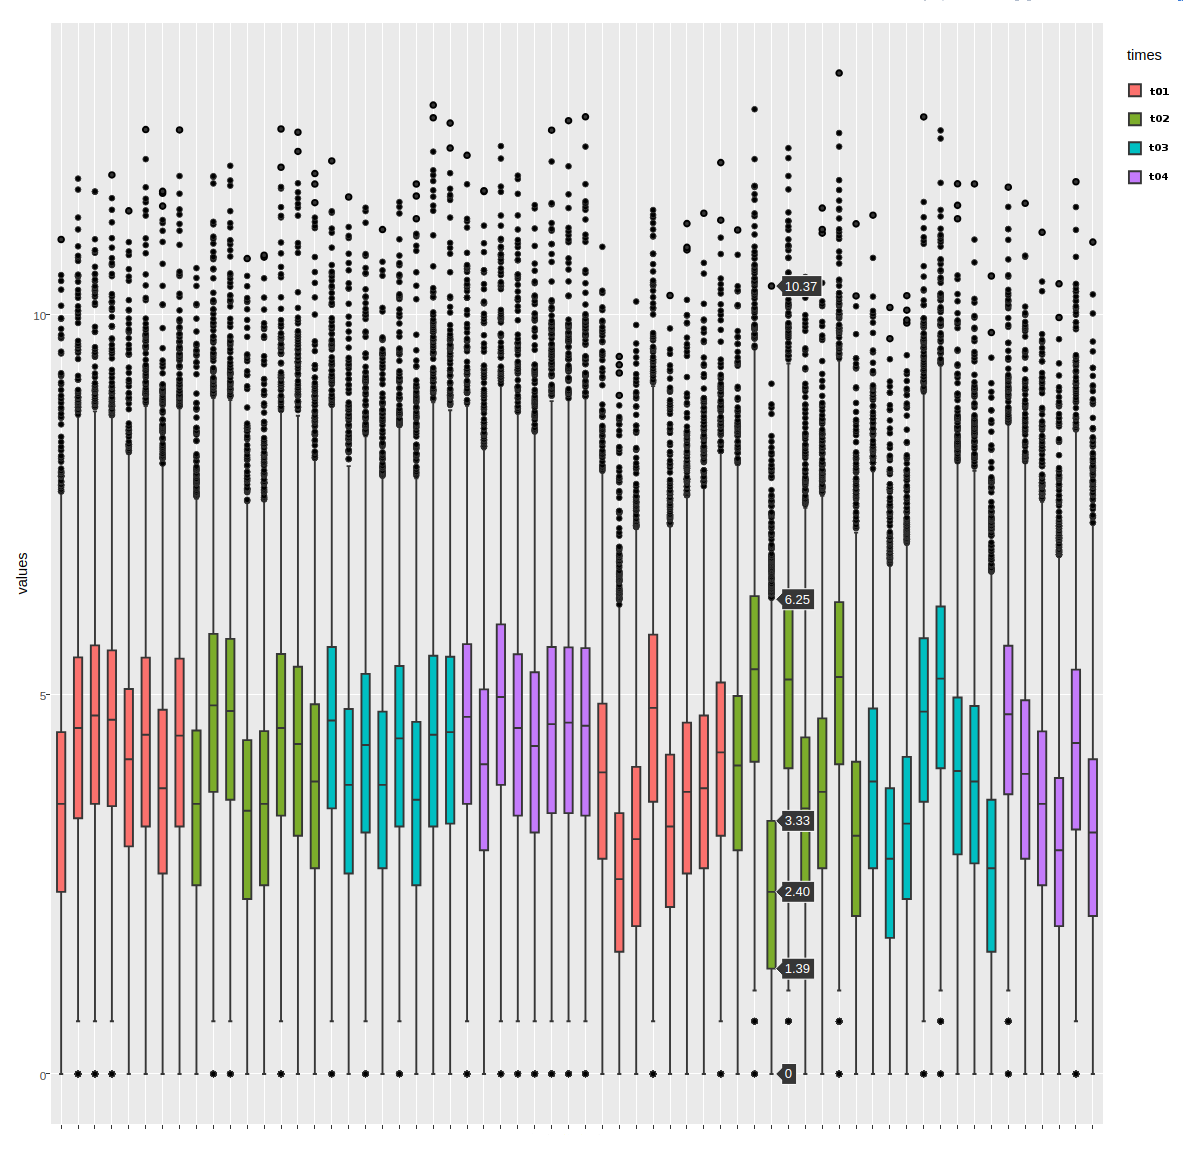
\includegraphics[width=\textwidth,height=\textheight,keepaspectratio]{img/ticorser/boxplot_example.png}
\caption[ticorser boxplot]{An example of interactive boxplot made with \gls{tic} package. Each boxplot represents a specific sample, while each colour represents a specific time point. When passing the mouse over a boxplot it shows additional information about its quartiles.}
\label{fig:ticorserboxplot}
\centering
\end{figure}
 

Due to the very high dimensionality of RNA-Seq data, it is widely considered common sense to apply the \gls{pca} dimensionality reduction technique, which allows to visualize the data limiting their representation to 2 or 3 dimensions.
There are several packages allowing to apply a \gls{pca} transformation, but we choose to implement it in the \lstinline!plotPCA! function, by using the \lstinline!prcomp! from the \textit{stats} package.
The user needs just to give the \lstinline!counts.data.frame! and the \lstinline!design.data.frame! by specifying the column name where to find the samples groups.
In such a way, the function will compute and plot the pca, colouring the samples according to the groups identified in the chosen column.
Moreover, by setting to \lstinline!TRUE! the \lstinline!ellipses! argument, the function will plot also the ellipses surrounding each samples group.


\begin{figure}[H]
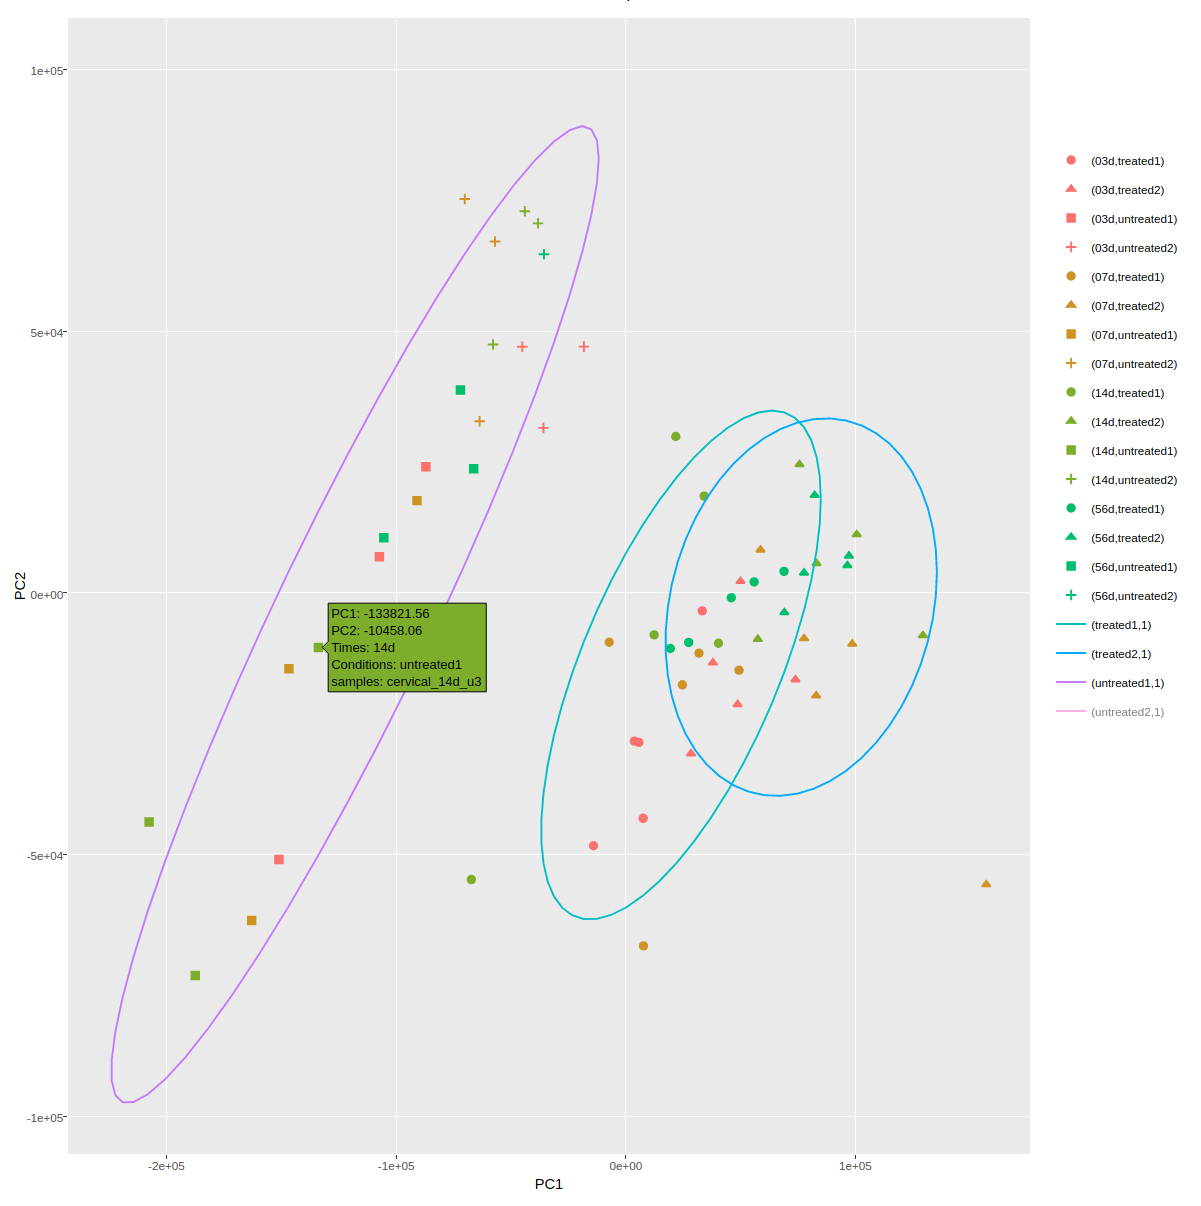
\includegraphics[width=\textwidth,height=\textheight,keepaspectratio]{img/ticorser/pca_example.png}
\caption[ticorser pca]{An example of interactive \gls{pca} made with \gls{tic} package. Each dot represents a specific sample, while each colour represents a time point, each simbol represents a biological condition group. When passing the mouse over a dot it shows additional information about the selected sample, while from the legend it's possible to show/hide groups or ellipses.}
\label{fig:ticorserpca}
\centering
\end{figure}

\subsubsection{DE Results Plots}
In order to inspect the results producted by DE methods, we implemented two kind of very common plots, the \textit{VolcanoPlot} and the \textit{MAPlot}.

Both our implementations takes as input a DE results data frame automatically recognizing which method produced it.
Moreover, it gives the possiblity to add a list of positive control genes, in order to annotate them on the volcano plot with a third colour.

The volcano plot puts in relation the $log_2(FC)$ with $log_{10}(p-value)$ in order to highlight the significant changes inside the data experiment.

\begin{figure}[H]
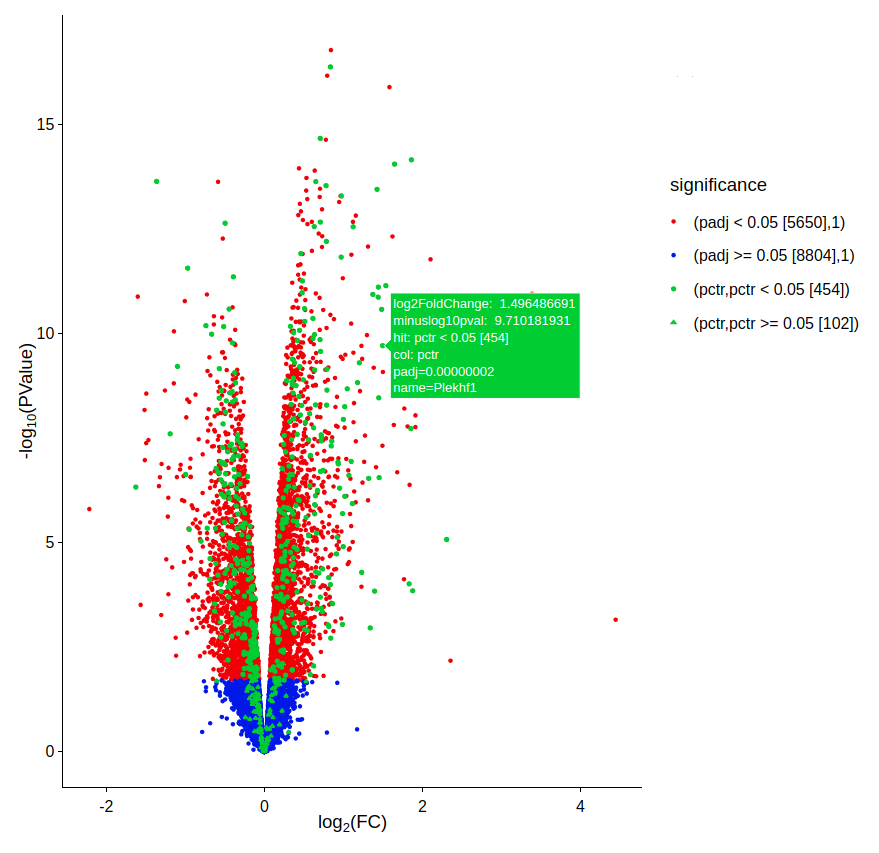
\includegraphics[width=\textwidth,height=\textheight,keepaspectratio]{img/ticorser/volcano_example.png}
\caption[ticorser volcano]{An example of interactive volcano plot made with \gls{tic} package. Each dot represents a gene, while blue and red colours highlights the significance of the genes. In green there are those genes coming from the positive control list. When passing the mouse over a dot it shows additional information about the selected gene.}
\label{fig:ticorservolcano}
\centering
\end{figure}

The MA-Plot puts in relation two quantities useful to understand the differences between the measurements in two conditions.
On the x-axis there is represented the $log_2(T/C)$ where \textit{T} is the treatement condition and \textit{C} its control.
It is not mandatory to have a DE results dataframe to plot an MA-plot, but it's pretty useful to have it in order to understand the distribution of the significant genes.
 

\begin{figure}[H]
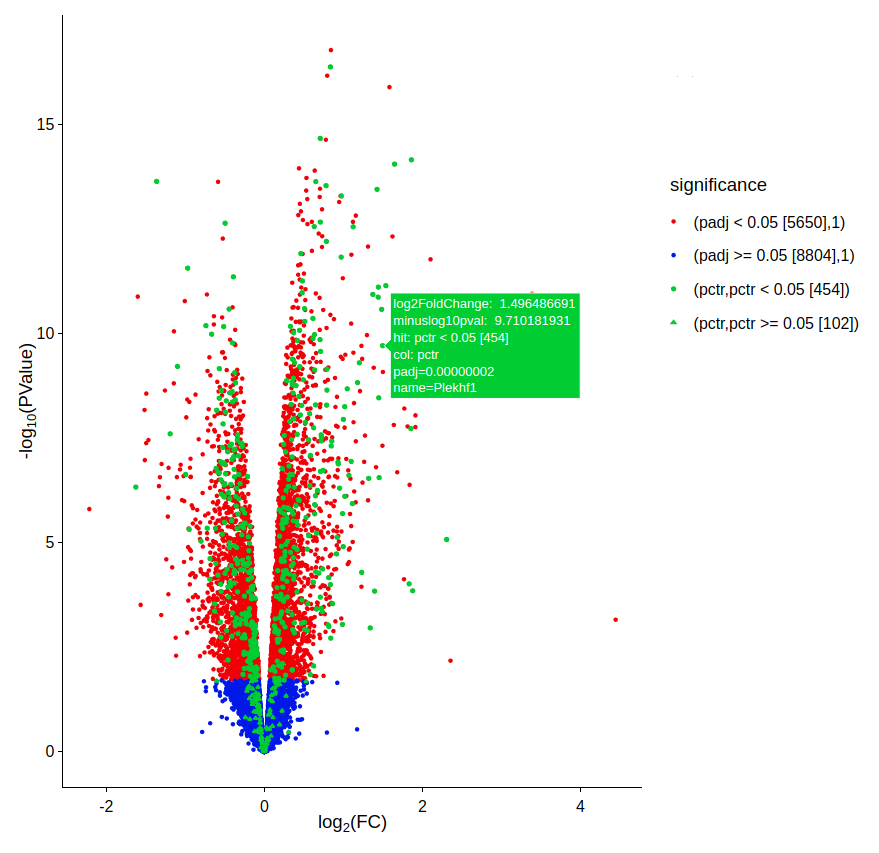
\includegraphics[width=\textwidth,height=\textheight,keepaspectratio]{img/ticorser/volcano_example.png}
\caption[ticorser MAplot]{An example of interactive MA-plot made with \gls{tic} package. Each dot represents a gene, while blue and red colours highlights the significance of the genes. When passing the mouse over a dot it shows additional information about the selected gene.}
\label{fig:ticorsermaplot}
\centering
\end{figure}


\subsubsection{Gene Profiles plot}
For highlighting the profile of a gene, we implemented the function \lstinline!plotGeneProfile!, where takes as input the count matrix, a gene name, and the design matrix.
In such a way the function is able to plot the profile of a gene showing its trend throught all time points, and between the different conditions.

\begin{figure}[H]
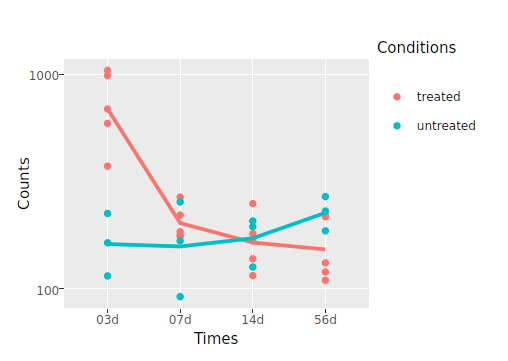
\includegraphics[width=\textwidth,height=\textheight,keepaspectratio]{img/ticorser/gene_trend.png}
\caption[ticorser gene profile]{An example of interactive gene profile made with \gls{tic} package. Each dot represents the counts value of the gene in a sample. Colours identifies the conditions of the samples. The lines represent the gene trend over all time points.}
\label{fig:ticorsergenetrend}
\centering
\end{figure}

\subsubsection{keggmap}
\gls{tic} offers the possibility to plot \textit{keggmaps}\cite{Kanehisa2016} taking into account the $log_2(FC)$ of the genes involved in the graphical representation, thought all the timepoints.
Indeed, using the \lstinline!plotKeggmap! function it enables to plot a \textit{keggmap}, using as input the counts and the design matrices, computing the $log_2(FC)$ at each time point, and showing it in the gene box inside the plot.

\begin{figure}[H]
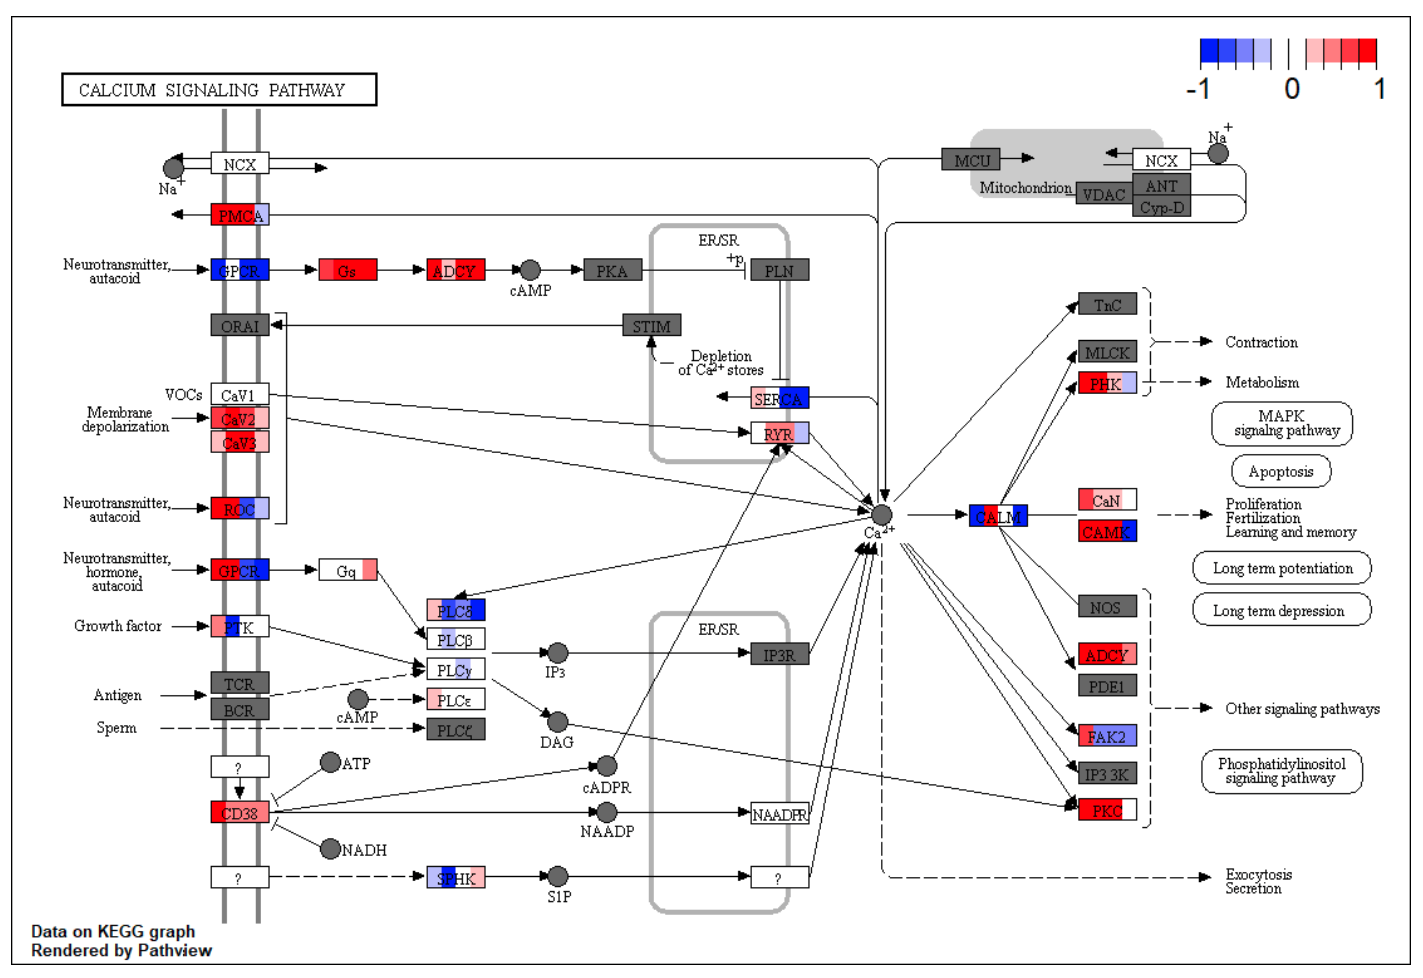
\includegraphics[width=\textwidth,height=\textheight,keepaspectratio]{img/ticorser/keggmap_example.png}
\caption[ticorser keggmap]{add description}
\label{fig:ticorserkeggmap}
\centering
\end{figure}








